

\begin{frame}{Heat From Information}
\begin{block}{The Second Law of Thermodynamics}
	\begin{itemize}
	\item Qualitatively, heat cannot flow from a cooler object to a hotter object.
	\item More Quantitatively, there exists a thermodynamic variable $S$, called the entropy, such that:
	\begin{equation*}
	0 \le S_f - S_0 + \Delta Q /T
	\end{equation*}	
	where the RHS of the inequality is called Entropy Production (EP).
	\item An increase in ``order" comes at the cost of producing Heat.
	\end{itemize}
\end{block}
\end{frame}


%Maxwell's demon diagram
\begin{frame}{Heat From Information}
\begin{figure}
	\centering
	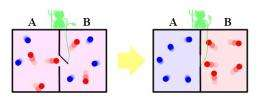
\includegraphics[scale=1]{../Images/maxwellsdemon.jpg}
	\caption{Maxwell's Demon}
	\label{fig:MaxwellsDemon}
\end{figure}
``\textit{... if we conceive of a being whose faculties are so sharpened that he can follow every molecule in its course, such a being, whose attributes are as essentially finite as our own, would be able to do what is impossible to us.}"\\
 \hspace{10mm} -- James Clerk Maxwell
\end{frame}

\begin{frame}{Heat From Information}
\begin{block}{Maxwell's Demon}
\begin{itemize}
	\item Small door can, in principle be opened with 0 EP.
	\item The location of each gas particle can be measured with 0 EP.
	\item Key lies in the demon's memory.
	\begin{itemize}
	\item The Demon must have finite memory.
	\item No matter how well-prepared, eventually the Demon must over-write (erase) one of its memory cells \parencite{bennett_thermodynamics_1982}.
	\end{itemize}
\end{itemize}
\end{block}
\end{frame}

\begin{frame}{Heat From Information}
\begin{block}{Landauer Cost}
\begin{itemize}
	\item The Boltzmann Entropy of a single information-carrying bit is $k\ln(2)$.
	\item The Boltzmann Entropy of a bit that has been erased is 0.
	\item By the second law:
	\begin{align*}
	0 &\le S_f - S_0 + \Delta Q /T\\
	\implies 0 &\le 0 -k\ln(2) + \Delta Q/T\\
	\implies kT\ln(2) & \le \Delta Q
	\end{align*}
	and we obtain the Landauer cost.
\end{itemize}
\end{block}
\end{frame}

%Analysis of Maxwell's Demon
